\chapter{Deriving Loewner's Equation}
\label{ch:proof}

In this appendix we shall give an overview of the demonstration of Loewner's
equation. For the mathematically inclined, a more detailed derivation can be
found in~\cite{delMonaco2013}. Let us do this~\cite{Kager2004}.

In Chapter~\ref{ch:sle} we defined the uniformizing map $g_t$ as a conformal
transformation that maps $\HH\setminus\gamma_{[0,t]}$ to $\HH$. The same way,
for a given $dt>0$ there is a map $g_{t-dt}$ that takes
$\HH\setminus\gamma_{[0,t-dt]}$ to $\HH$. We define a transition map
$G_{t,dt}=g_t\circ g_{t-dt}^{-1}$ that maps
$\HH\setminus\gamma_{[0,t-dt]}$ to $\HH\setminus\gamma_{[0,t]}$. For a
reference of the relationship between these functions see
Fig.~\ref{fig:proofscheme}.


We use the fact that a conformal map $f(z)$ is completely defined by its value
on the boundary (which in the case of the upper half plane is the real line).
The value of the function on the whole domain can be recovered by using the
Schwartz integral formula~\cite{Ahlfors1979}
\begin{equation}
    f\left(z\right)=
    \frac{1}{\pi}\int_{-\infty}^{\infty}
    \frac{\mbox{Im }f\left(\xi\right)}{\xi-z}d\xi.
\end{equation}
Since $\mbox{Im}\{\xi - f(z)\}=-\mbox{Im }f(z)$ for $\xi$ real we can write
\begin{equation}
    z-G_{t,dt}^{-1}\left(z\right)=
    \frac{1}{\pi}\int_{a}^{b}
    \frac{\mbox{Im }G_{t,dt}^{-1}\left(\xi\right)}{z-\xi}d\xi.
\end{equation}
Where the interval $[a,b]$ is the (assumed finite) region where $\mbox{Im
}G_{t,dt}^{-1}(z)>0$. Making the substitution
$z\rightarrow G_{t,dt}(z)$ we obtain
\begin{equation}
    \label{eq:proof1}
    G_{t,dt}\left(z\right)-z=
    \frac{1}{\pi}\int_{a}^{b}
    \frac{\mbox{Im }G_{t,dt}^{-1}\left(\xi\right)}
    {G_{t,dt}\left(z\right)-\xi}d\xi.
\end{equation}
Multiplying both sides by $z$ and taking the limit $z\rightarrow\infty$ we
obtain a formula for the half plane capacity
\begin{equation}
    a_{t,dt}=\frac{1}{\pi}\int_{a}^{b}
    \mbox{Im }G_{t,dt}^{-1}\left(\xi\right)d\xi.
\end{equation}
As mentioned in Section~\ref{sec:le}, the choice of capacity is mostly arbitrary, but a
common choice is
\begin{equation}
    a_t = 2t,
\end{equation}
which, based on the additivity property
\begin{equation}
    a_t = a_{t-dt} + a_{t,dt},
\end{equation}
yields the relation
\begin{equation}
    \label{eq:proof2}
    \int_{a}^{b}\mbox{Im }G_{t,dt}^{-1}\left(\xi\right)d\xi=2\pi dt.
\end{equation}

We can now tackle the time derivative of the uniformizing map $g_t$
\begin{equation}
    \frac{\partial g_{t}\left(z\right)}{\partial t}=
    \lim_{dt\rightarrow0}\frac{g_{t}\left(z\right)-g_{t-dt}\left(z\right)}{dt}.
\end{equation}
Using the fact that $g_{t}=G_{t,dt}\left(g_{t-dt}\left(z\right)\right)$,
and Eqs.~\ref{eq:proof1} and~\ref{eq:proof2} we obtain
\begin{equation}
    \frac{\partial g_{t}\left(z\right)}{\partial t}=
    \lim_{dt\rightarrow0}\frac{2}
    {\int_{a}^{b}\mbox{Im }G_{t,dt}^{-1}\left(\xi\right)d\xi}
    \int_{a}^{b}
    \frac{\mbox{Im }G_{t,dt}^{-1}\left(\xi\right)}
    {G_{t,dt}\left(g_{t-dt}\left(z\right)\right)-\xi}d\xi.
    \label{eq:proof4}
\end{equation}
The second mean value theorem~\cite{Comenetz2002} for definite integrals states that
it exists a $c\in\left(a,b\right]$ such that
\begin{equation}
    \int_{a}^{b}G\left(\xi\right)f\left(\xi\right)d\xi=
    \lim_{y\rightarrow a^+}G\left(y\right)\int_{a}^{c}f\left(\xi\right)d\xi.
\end{equation}
Applying that to Eq.~\ref{eq:proof4} leaves us with
\begin{equation}
    \label{eq:proof3}
     \frac{\partial g_{t}\left(z\right)}{\partial t}=
     \lim_{dt\rightarrow0}
     \frac{2}{G_{t,dt}\left(g_{t-dt}\left(z\right)\right)-a}
     \frac{\int_{a}^{c}\mbox{Im }G_{t,dt}^{-1}\left(\xi\right)d\xi}
          {\int_{a}^{b}\mbox{Im }G_{t,dt}^{-1}\left(\xi\right)d\xi}.
\end{equation}
Since in the limit of $dt\rightarrow0$, $\mbox{Im }G_{t,dt}^{-1}(z)$ is
zero except for $z=U_t$, in other words, $a=b=U_t$. This means that the two
integrals in Eq.~\ref{eq:proof3} take the same value and cancel each other. Add
the fact that $\lim_{dt\rightarrow 0}G_{t,dt}$ is the identity map, and
this leaves us with Loewner's equation
\begin{equation}
    \frac{\partial g_t(z)}{\partial t} = \frac{2}{g_t(z) - U_t}.
\end{equation}

\begin{figure}
\begin{center}
    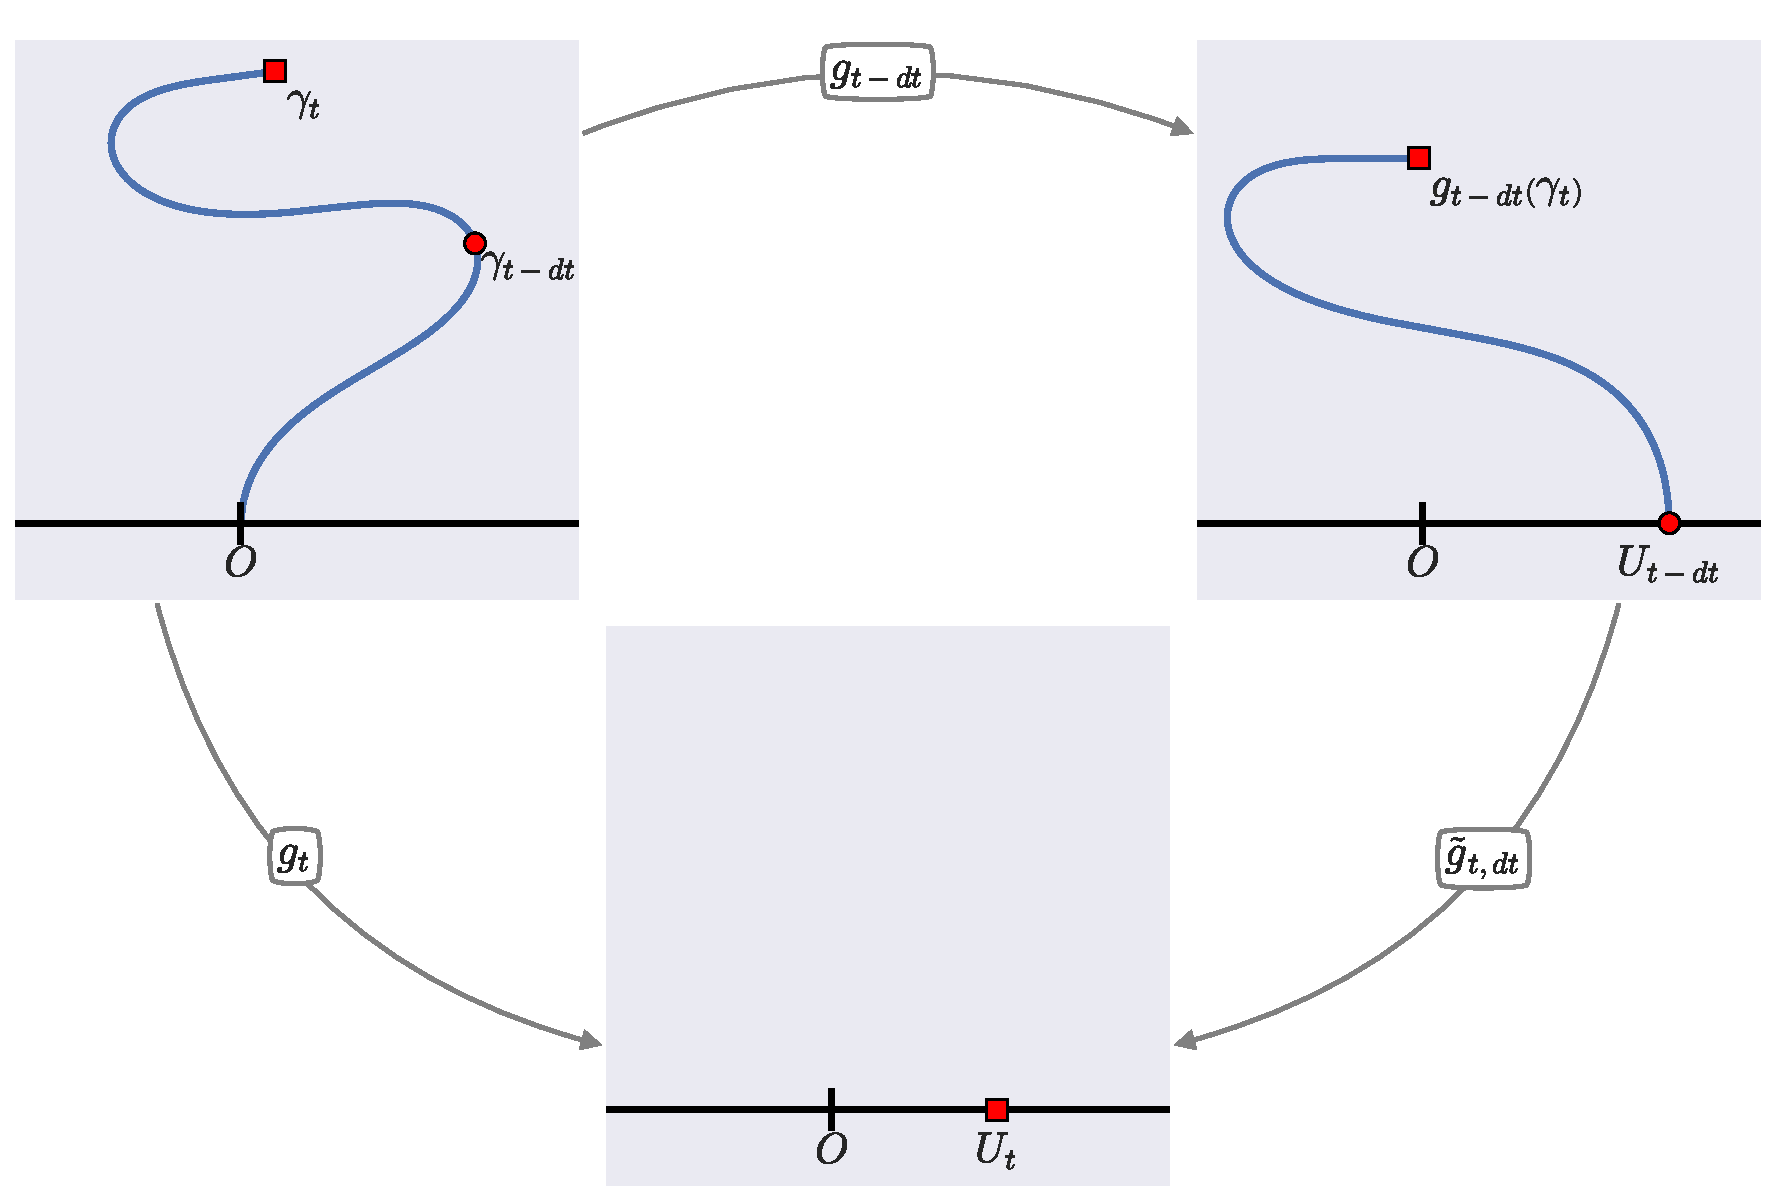
\includegraphics[scale=0.4]{chapters/ch7-apdx/figs/proofscheme}
\end{center}
\caption{Construction of the transition map $G_{t,dt}=g_t\circ
    g_{t-dt}^{-1}$. The interval $[a,b]$ is the region where
    $\mbox{Im }G_{t,dt}(z)>0$.}
\label{fig:proofscheme}
\end{figure}
